\section{Remedies, scored on the same tracks}\label{sec:remedies}

The literature's corrections were built for the end strips without saying so. We score each of them, and the charge-weighted
time, on the same 50\,000 projections against the reference, with two figures of merit: the median steepness bias in bins of
the reference angle (the median of the signed angle error times the sign of the reference angle, so that the compression does
not cancel between the two track directions) and the angle resolution $s_{68}$ (the 68th percentile of the absolute error about
the median within \ang{5}) after a global linear calibration of the slope on the other half of the events. The second figure is
what a $\mu$TPC with a calibration run achieves; the first is what it suffers without one. \Cref{tab:remedies} gives both for
Run 1; Run 2 agrees within 0.1 to 0.2 degrees throughout. The corrections are:

\begin{description}
\item[robust line] iterative $3\sigma$ trimming of strips about the line, the role of the Hough step in the NSW and APV25 chains;
\item[edge cut] the first or last strip dropped when its amplitude is below 1/2~\cite{Rinnagel2019}, 1/4 or 1/6~\cite{Sessa2014} of the
  inner neighbour's: the ghost-hit cut;
\item[edge shift] the kept edge strip moved inward by $(1 - a_{\rm edge}/a_{\rm inner})\,p/2$, the centroid of the partial column
  it collects: the geometric correction of Ntekas and Farinelli~\cite{Ntekas2016,Farinelli2019} in a form that needs no calibration;
\item[neighbour subtraction] $W_i \to W_i - f\,(W_{i-1} + W_{i+1})$ sample by sample before the hit is formed, with $f = 0.07$ (the
  same-time floor of \cref{sec:phase}), 0.15~\cite{Loesel2017,Flierl2018}, 0.20~\cite{Flierl2018} and 0.30~\cite{Herrmann2019};
\item[charge-weighted time] the centroid in time of the pulse above threshold, the estimator of the pad TPCs, which the formulation
  predicts to remove the interior term.
\end{description}

\begin{table}[t]
  \centering\footnotesize
  \caption{Hit-level remedies on chamber A, Run 1, against the reference: implied drift velocity of the raw ladder (true
  \SI{37.1}{} X / \SI{36.3}{\micro\metre/ns} Y), median steepness bias per angle bin without calibration, and the angle resolution
  after a global scale calibration. V0 is the leading-edge hit; ``template'' the per-strip matched-filter time; ``cw'' the
  charge-weighted time. H2c is the forward model of \cref{sec:forward} fitted to the hit lists; W the forward fit of the
  waveforms~\cite{paperII}.}
  \label{tab:remedies}
  \begin{tabular}{@{}llcccccc@{}}
    \toprule
    & & implied $v$ & \multicolumn{4}{c}{steepness bias [\si{\degree}] at $|\tan\theta|$ =} & $s_{68}$ [\si{\degree}] \\
    view & reading & [\si{\micro\metre/ns}] & 0.05--0.1 & 0.1--0.2 & 0.2--0.3 & 0.3--0.5 & calibrated \\
    \midrule
    X & V0 leading edge & 44.8 & 3.46 & 2.47 & 1.64 & 1.43 & 2.06 \\
      & V0 + robust line & 44.1 & 3.38 & 2.32 & 1.51 & 1.21 & 2.05 \\
      & V0 + edge cut 1/2 & 43.4 & 3.09 & 2.12 & 1.36 & 1.08 & 1.97 \\
      & V0 + edge cut 1/6 + edge shift & 43.6 & 3.16 & 2.16 & 1.42 & 1.15 & 1.97 \\
      & V0 + 15\,\% subtraction + robust & 41.1 & 2.40 & 1.46 & 0.96 & 0.76 & 1.69 \\
      & V0 + 15\,\% subtraction + edge shift & 40.3 & 2.02 & 1.25 & 0.82 & 0.74 & 1.54 \\
      & V0 + 30\,\% subtraction & 39.2 & 1.72 & 0.92 & 0.62 & 0.53 & 1.51 \\
      & charge-weighted time + robust & 44.9 & 3.61 & 2.48 & 1.59 & 1.23 & 2.26 \\
      & charge-weighted + 30\,\% subtraction & 38.6 & 1.69 & 0.69 & 0.39 & 0.48 & 1.60 \\
      & template time + 15\,\% + edge shift & 39.9 & 1.87 & 1.09 & 0.69 & 0.57 & 1.55 \\
      & H2c: forward model on hit lists & & \multicolumn{4}{c}{$-0.05$ overall} & 1.20 \\
      & W: forward fit of the waveforms & & $-0.02$ & $0.00$ & $-0.06$ & $+0.02$ & 1.04 \\
    \midrule
    Y & V0 leading edge & 51.5 & 4.18 & 3.21 & 1.98 & 1.40 & 2.68 \\
      & V0 + robust line & 47.2 & 3.85 & 2.50 & 1.43 & 0.94 & 2.42 \\
      & V0 + edge cut 1/2 & 46.8 & 3.71 & 2.40 & 1.36 & 0.87 & 2.40 \\
      & V0 + 15\,\% subtraction + robust & 42.8 & 2.69 & 1.48 & 0.78 & 0.38 & 1.98 \\
      & V0 + 30\,\% subtraction & 45.6 & 3.39 & 2.07 & 1.10 & 0.90 & 2.32 \\
      & charge-weighted time + robust & 47.6 & 3.09 & 1.96 & 1.09 & 0.80 & 2.66 \\
      & charge-weighted + 15\,\% + robust & 42.9 & 2.34 & 1.13 & 0.43 & 0.32 & 2.30 \\
      & template time + 15\,\% + edge shift & 41.9 & 2.28 & 1.16 & 0.47 & 0.21 & 2.02 \\
      & H2c: forward model on hit lists & & \multicolumn{4}{c}{$+0.19$ overall} & 1.28 \\
      & W: forward fit of the waveforms & & $+0.03$ & $0.00$ & $+0.05$ & $+0.04$ & 1.01 \\
    \bottomrule
  \end{tabular}
\end{table}

\begin{figure}[t]
  \centering
  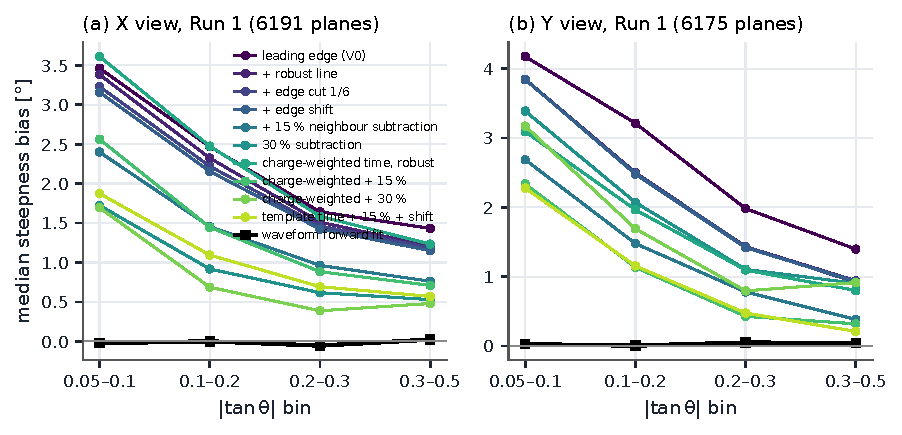
\includegraphics[width=\linewidth]{remedies_bias}
  \caption{Median steepness bias against the reference angle for the leading-edge hits with each correction, the
  charge-weighted time, and the forward fit of the waveforms (black), Run 1, X (a) and Y (b).}
  \label{fig:remedies}
\end{figure}

Four things follow (\cref{fig:remedies}).

\emph{The edge treatments act where the bias is and remove a quarter of it.} Cutting or shifting the edge strips lowers the
raw bias by 10 to 15\,\% at every angle on X and brings the calibrated resolution from \ang{2.06} to \ang{1.97}; the toy
(\cref{app:toy}) predicts a 24\,\% reduction of $C$ from the edge shift alone, with the difference made up by the real
chamber's ghosts, which the charge-ratio cut does not catch when they carry a few per cent of the centre strip at the
same time as it.

\emph{The neighbour subtraction is the strongest single correction, and its best factor is not a capacitance.} Subtracting
15\,\% of the neighbours' samples halves the calibrated resolution gap on X (\ang{1.69}) and Y (\ang{1.98}); 30\,\% does better on X
(\ang{1.51}, bias 0.5 to \ang{1.7}) but worse on Y (\ang{2.32}), where the neighbours' signals are the delayed resistive charge and
subtracting them at the same time removes real charge. The factor that restores the angle on X, 30\,\%, is Flierl's and
Herrmann's~\cite{Flierl2018,Herrmann2019}, and it is four to five times the same-time coupling that the waveforms allow
(\cref{sec:phase}): it deconvolves every same-time share in the ladder, the Gaussian footprint and the diffusion included, and
compensates the rest by over-correction. Herrmann's observation that even 40\,\% does not restore the expected first-to-last
time difference~\cite{Herrmann2019} is what one expects of a nearest-neighbour subtraction applied to a spread that reaches the
second neighbour and grows with depth.

\emph{The charge-weighted time does nothing by itself.} It reads the same compression as the leading edge on X (\ang{2.52} against
\ang{2.48} raw) and a worse one on Y (\ang{3.05}), where the delayed resistive charge pulls a centroid later on the strips it
reaches. It becomes the best estimator only after the subtraction (\ang{1.78} raw, \ang{1.28} on Y with 15\,\%), because the
subtraction removes the end charge and leaves an interior that the centroid reads without compression. The prediction of
\cref{sec:formulation} holds, and it is a statement about the interior term, which here is small.

\emph{No hit-level recipe closes the gap to the waveform fit.} The best combination on each view, 30\,\% subtraction on X and
charge-weighted time with 15\,\% subtraction on Y, leaves the calibrated resolution at \ang{1.5} to \ang{2.0} against \ang{1.0} for the
forward fit of the waveforms, and a residual bias of \ang{0.5} to \ang{2.3} without a calibration run. The forward model fitted
to the hit lists alone (H2c, one time and one amplitude per strip, the physics of the waveform fit and nothing of its
samples~\cite{paperII}) reaches \ang{1.20}/\ang{1.28}: most of the remaining gap is information the hits do not keep, not
knowledge the corrections lack.

\subsection{The forward model}\label{sec:forward}

The alternative to correcting the hit times is not to form them. \Cref{eq:waveform} is linear in the charge profile $q(u)$ for
a given track, so with the lateral spreads and the impulse response calibrated once per detector and run condition, the whole
strip-by-sample picture of an event can be predicted for a trial $(x_0, w, t_0)$ and the profile solved by non-negative least
squares; the track parameters are then the minimum of the $\chi^2$ over all samples of all strips~\cite{paperII}. The neighbours'
shares, same-time or delayed, are part of the prediction and stop being contamination; the partial strips and the ghosts are
predicted with the charge the model puts there and weigh in the fit by their information, not by a cut. The method is the
$\mu$TPC analogue of the simultaneous multi-pad waveform fit with which T2K maps its resistive spreading~\cite{T2K2023} and of
the channel-and-time convolution model of the liquid-argon deconvolution~\cite{Adams2018a}; what is new is that the drift-depth
profile is solved inside the fit, which is what turns a sharpened centroid into a track segment. On chamber A it reads the
reference slope to 1\,\% at every angle (\cref{fig:universal}a) with a resolution of \ang{1.0}, against a diffusion-limited floor of
\ang{0.3}~\cite{paperII}; on the re-simulated arms it stays within 1\,\% of the truth up to ten times the resistive spreading and for
every footprint and diffusion tried, because the mixing is in the model.

Its cost is the waveform: a sampled front end with enough samples to cover the column and the impulse response (here 32 at
\SI{60}{ns}), the calibration of the spreads per detector and run condition, and about a second of CPU per projection. A
hit-only front end that keeps one time and one amplitude per strip recovers most of the resolution gap only through the same
model (H2c), and none of it through corrections of the hit times.
